\section{Versuchsaufbau/-durchführung}
In dem Versuch sollen zwei Proben (Kupfer und Zink) auf den \emph{Hall-Effekt} untersucht werden. %Zink

\subsection{Hysteresemessung}
Die Hysteresemessung dient dazu, die Abhängigkeit der Magnetfeldstärke
von der Stromstärke zu bestimmen.
Gleichzeitig soll aber auch die Auswirkung der Hysterese untersucht werden.
 Der Versuch wird wie in \ref{fig: auf_hall} zu sehen aufgebaut, %Kommata oder Satz anders formulieren
mit Hilfe eines Teslameters wird für zehn verschiedene Stromstärken das Magnetfeld bestimmt. %Mit Hilfe
Die ersten zehn Messungen werden beim Hochfahren des Magneten getätigt, %Komma; $10$ bzw zehn konsistent
die anderen zehn beim Herunterfahren.

\begin{figure}
  \centering
  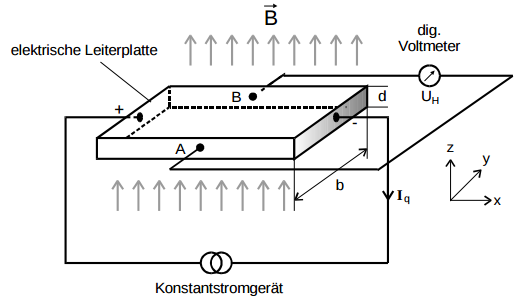
\includegraphics[width=0.7\textwidth]{pics/Halleffekt_aufbau.png}
  \caption{Versuchsaufbau für die Messung der Hallspannung}
  \label{fig: auf_hall}
\end{figure}

\begin{center}
Die im Folgenden beschriebenen Messungen werden immer zwei Mal durchgeführt. % - komma
Beim zweiten Durchgang wird die Spannung umgepolt. %Stil
Dies dient zur Vermeidung von systematischen Fehlern (z.\,B. Störspannung). %z.\,B.
\end{center}

\subsection{Bestimmung des Widerstands}
Zur Widerstandsbestimmung werden ein Voltmeter und
eine Spannungsquelle benötigt.
Nachdem beide an die Probe angeschlossen sind,
wird die Spannungsquelle eingeschaltet und die Stromstärke variiert.
Für jede Probe wird zu zehn verschiedenen Stromstärken
die Spannung am Voltmeter notiert.
Mithilfe des ohmschen Gesetzes kann dann auf den Widerstand geschlossen werden.

\subsection{Messung der Hallspannung}
Der grundlegende Versuchsaufbau ist in Abbildung \ref{fig: auf_hall} dargestellt.
Zunächst werden die Abmessungen (Breite, Höhe und Länge) der Probe gemessen.
Anschließend folgt die Verkabelung nach dem in \ref{fig: kabel_hall} abgebildeten Schaltbild.
Die verkabelte Probe wird nun in eine Haltevorrichtung befestigt. Diese sorgt dafür, dass %gegeben passt nicht gut; dafür
der Stromfluss durch die Probe orthogonal zum Magnetfeld steht.
Für die Messung der \emph{Hall-Spannung} gibt es nun zwei Verfahren.
Zum einen kann die Stromstärke, die an der Probe anliegt konstant gelassen werden und
die Magnetfeldstärke variiert werden. Zum Andern kann
aber auch die Magnetfeldstärke konstant gelassen werden und die Stromstärke verändert
werden. Für beide Verfahren sollten zehn Messpunkte gewählt werden.
Bei der Regelung des Elektromagneten ist darauf zu achten, dass der
erzeugende Strom langsam heruntergefahren wird.
Die von dem Hall-Effekt erzeugt Spannugn kann dann wie folgt berechnet werden: %erzeugte Spannung
\begin{equation} %Füg hier besser die fertige Formel ein 
\label{eq:hall_spann}
U\ua{H}=\frac{1}{2}\left(U\ua{ges+}-U\ua{ges-}\right)
\end{equation}

\begin{figure}
  \centering
  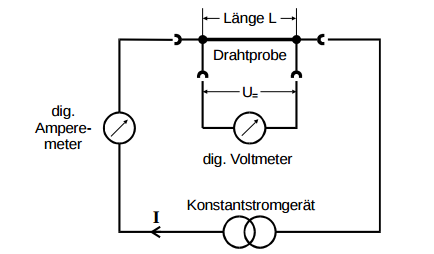
\includegraphics[width=0.7\textwidth]{pics/verkabelung_hall.png}
  \caption{Verkabelung für die Messung der Hallspannung}
  \label{fig: kabel_hall}
\end{figure}
